% ============================================================
% CHAPTER 4: IMPLEMENTATION DETAILS
% ============================================================

\chapter{IMPLEMENTATION DETAILS}
\label{chap:implementation}

This chapter translates the architectural blueprint from Chapter~\ref{chap:architecture} into executable code. It presents the core algorithms with real source listings, documents the concurrency model, and addresses the engineering challenges of Android OEM fragmentation and high-throughput garbage collection.

% ────────────────────────────────────────────────────────────
\section{Development Environment}
\label{sec:dev_environment}

\begin{table}[H]
\centering
\caption{Technology Stack Overview}
\label{tab:tech_stack}
\begin{tabularx}{\textwidth}{l l X}
\toprule
\textbf{Component} & \textbf{Technology} & \textbf{Purpose} \\
\midrule
Language        & Kotlin 1.9+            & Primary language; null safety, coroutines \\
UI Framework    & Jetpack Compose        & Declarative Android UI \\
Min SDK         & Android 10 (API 29)    & Required for \texttt{getConnectionOwnerUid()} \\
Concurrency     & Kotlin Coroutines      & Lightweight I/O multiplexing \\
Server          & Node.js 18+ / Express  & RESTful backend \& telemetry ingestion \\
Database        & sql.js (SQLite/WASM)   & Embedded storage \\
Visualization   & Chart.js 4.x           & Real-time dashboard charts \\
\bottomrule
\end{tabularx}
\end{table}

\begin{figure}[H]
\centering
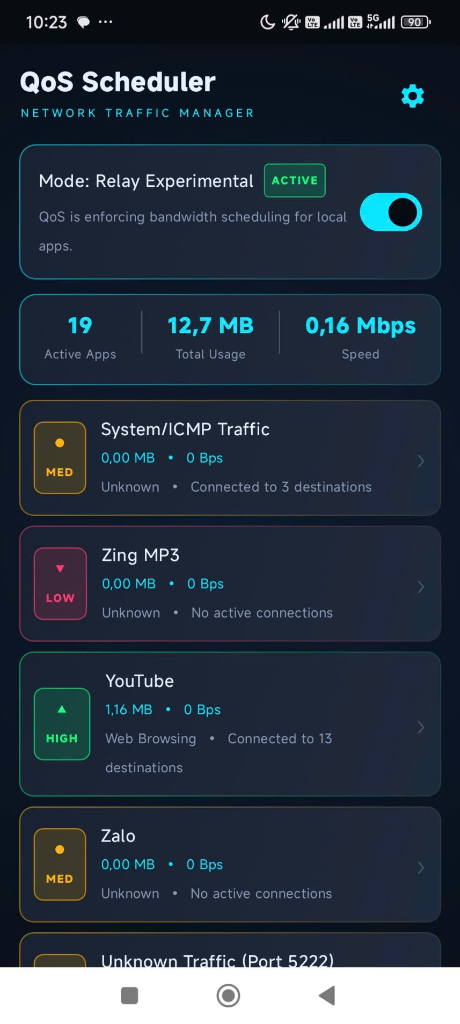
\includegraphics[width=0.45\textwidth]{figures/app_ui.png}
\caption{QoS Scheduler Android application built with Jetpack Compose.}
\label{fig:android_app_ui}
\end{figure}

% ────────────────────────────────────────────────────────────
\section{VPN and TUN Implementation}
\label{sec:vpn_implementation}

\subsection{TUN Interface Configuration}

The \texttt{QosVpnService} creates a dual-stack TUN interface capturing all device traffic:

\begin{lstlisting}[language=Java, caption={TUN interface configuration with dual-stack support}, label={lst:vpn_builder}]
val builder = Builder()
    .setSession("QoS Scheduler")
    .addAddress("10.0.0.2", 24)        // Virtual IPv4
    .addAddress("fd00::2", 128)        // Virtual IPv6
    .addRoute("0.0.0.0", 0)           // Capture all IPv4
    .addRoute("::", 0)                 // Capture all IPv6
    .setMtu(1500)                      // Standard Ethernet MTU
    .setBlocking(true)

val tunFd = builder.establish()
    ?: throw IllegalStateException("VPN permission not granted")
\end{lstlisting}

The routes \texttt{0.0.0.0/0} and \texttt{::/0} redirect \textit{all} traffic through TUN. MTU is set to 1500 bytes to prevent IP fragmentation.

\subsection{Packet Interception Loop}

The read loop runs on \texttt{Dispatchers.IO} to avoid blocking the UI thread:

\begin{lstlisting}[language=Java, caption={Packet interception loop with buffer reuse}, label={lst:intercept_loop}]
coroutineScope.launch(Dispatchers.IO) {
    val inputStream = FileInputStream(tunFd.fileDescriptor)
    val buffer = ByteArray(1500) // Reused MTU-sized buffer

    while (isActive) {
        val length = inputStream.read(buffer)
        if (length > 0) {
            dataPlaneProcessor.process(buffer.copyOfRange(0, length))
        }
    }
}
\end{lstlisting}

A \texttt{SupervisorJob} scopes all concurrent tasks (interception, app observer, telemetry push) to the service lifecycle, ensuring one child's failure does not cancel siblings.

% ────────────────────────────────────────────────────────────
\section{Packet Parsing (Data Plane)}
\label{sec:impl_data_plane}

Parsing extracts the 5-tuple in $O(1)$ using bitwise operations to avoid object allocation during high-throughput periods.

\subsection{IPv4 Header Extraction}

\begin{lstlisting}[language=Java, caption={IPv4 5-tuple extraction via bitwise operations}, label={lst:bitwise_parse}]
// IP Version: upper 4 bits of byte 0
val version = (data[0].toInt() shr 4) and 0x0F

// Header Length: lower 4 bits of byte 0, in 32-bit words
val ihl = (data[0].toInt() and 0x0F) * 4

// Protocol: byte 9 (6=TCP, 17=UDP)
val protocol = data[9].toInt() and 0xFF

// Source IP: bytes 12-15, Destination IP: bytes 16-19
val srcIp = InetAddress.getByAddress(data.copyOfRange(12, 16)).hostAddress
val dstIp = InetAddress.getByAddress(data.copyOfRange(16, 20)).hostAddress

// Transport ports: 2 bytes big-endian at IHL offset
val srcPort = ((data[ihl].toInt() and 0xFF) shl 8) or
              (data[ihl + 1].toInt() and 0xFF)
val dstPort = ((data[ihl + 2].toInt() and 0xFF) shl 8) or
              (data[ihl + 3].toInt() and 0xFF)
\end{lstlisting}

IPv6 parsing follows a separate code path: the fixed 40-byte base header is followed by an extension header chain traversed via the ``Next Header'' field until the transport protocol (TCP/UDP) is reached.

\subsection{UID Resolution}

The \texttt{AppResolver} maps 5-tuples to application UIDs via \texttt{getConnectionOwnerUid()}, using a multi-tier cache to amortize the expensive system call:

\begin{lstlisting}[language=Java, caption={Multi-tier UID resolution with negative caching}, label={lst:uid_resolve}]
fun resolveUid(srcIp: String, srcPort: Int,
               dstIp: String, dstPort: Int, protocol: Int): Int {
    val key = "$srcIp:$srcPort-$dstIp:$dstPort/$protocol"

    // Tier 1: Positive cache
    uidCache[key]?.let { return it }
    // Tier 2: Negative cache (known unresolvable)
    if (negativeCache.containsKey(key)) return -1

    // Tier 3: Kernel system call
    val uid = connectivityManager.getConnectionOwnerUid(
        protocol, InetSocketAddress(srcIp, srcPort),
        InetSocketAddress(dstIp, dstPort)
    )
    if (uid >= 0) { uidCache[key] = uid; return uid }

    // Promote to negative cache after 3 failures
    val fails = failCountCache.compute(key) { _, v -> (v ?: 0) + 1 } ?: 1
    if (fails >= 3) { negativeCache[key] = true; failCountCache.remove(key) }
    return -1
}
\end{lstlisting}

% ────────────────────────────────────────────────────────────
\section{Scheduling Engine}
\label{sec:impl_scheduler}

\subsection{Token Bucket with Lazy Refill}

The \texttt{TokenBucket} uses on-demand token computation (no background timer) with nanosecond precision:

\begin{lstlisting}[language=Java, caption={Token Bucket: lazy refill with synchronized access}, label={lst:token_bucket}]
class TokenBucket(
    @Volatile var rateBps: Long,   // Token fill rate (bits/sec)
    @Volatile var burstBits: Long  // Maximum capacity (bits)
) {
    private var tokens: Double = burstBits.toDouble()
    private var lastRefillTime: Long = System.nanoTime()

    @Synchronized
    fun consume(bytes: Int): Boolean {
        refill()
        val bitsNeeded = bytes.toDouble() * 8.0
        return if (tokens >= bitsNeeded) {
            tokens -= bitsNeeded
            true  // ALLOWED
        } else {
            false // DROPPED
        }
    }

    private fun refill() {
        val now = System.nanoTime()
        val elapsed = (now - lastRefillTime) / 1_000_000_000.0
        tokens = minOf(burstBits.toDouble(), tokens + rateBps * elapsed)
        lastRefillTime = now
    }
}
\end{lstlisting}

The \texttt{minOf} call caps tokens at burst capacity, preventing uncontrolled spikes after idle periods.

\begin{figure}[H]
\centering
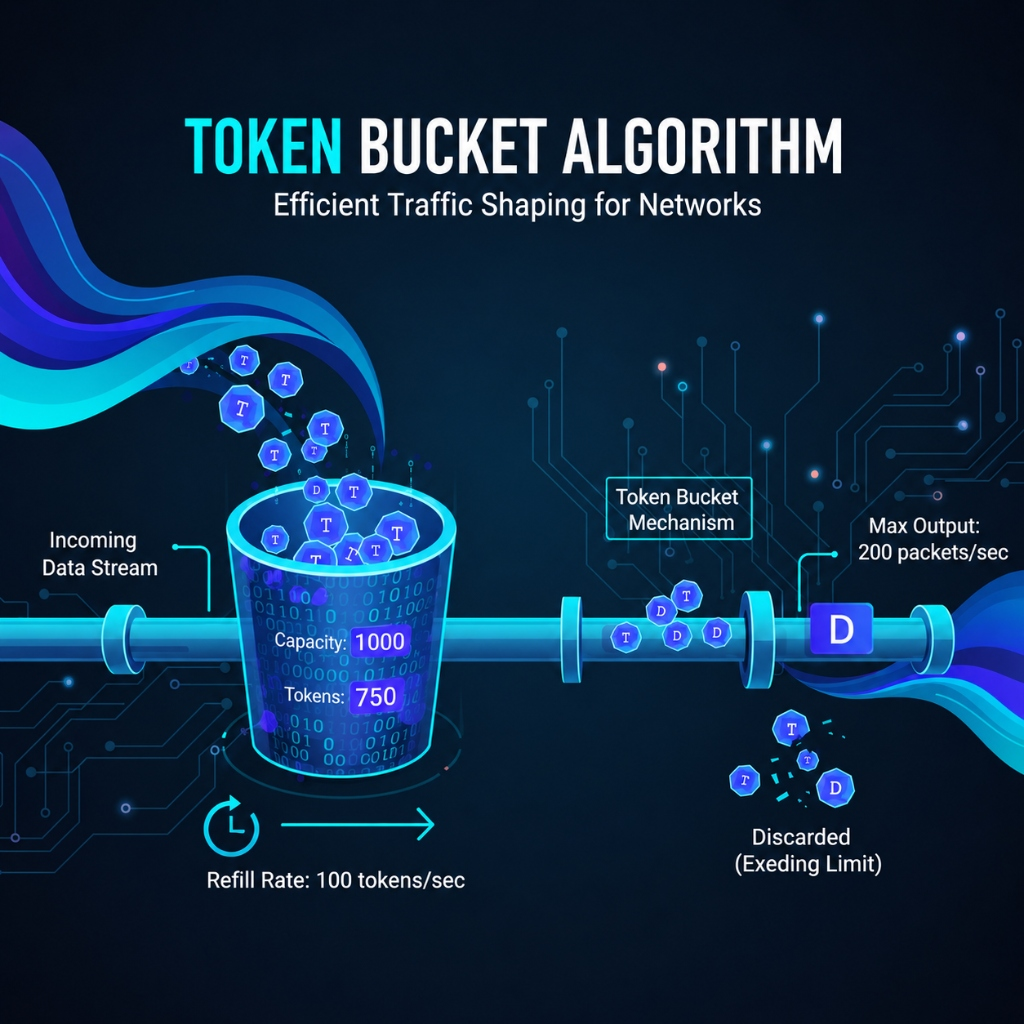
\includegraphics[width=0.85\textwidth]{figures/token_bucket_diagram.jpg}
\caption{Token Bucket algorithm: token refill, burst capacity, and packet consumption.}
\label{fig:token_bucket_impl}
\end{figure}

\subsection{WFQ Rebalance Algorithm}

The \texttt{BandwidthScheduler} dynamically adjusts Token Bucket rates using the GPS formula (Equation~\ref{eq:gps}):

\begin{lstlisting}[language=Java, caption={WFQ rebalance: bandwidth allocation by priority weight}, label={lst:wfq_rebalance}]
fun rebalanceWithApps(apps: Collection<AppTraffic>) {
    val highCount = apps.count { it.priorityClass == TrafficClass.HIGH }
    val medCount  = apps.count { it.priorityClass == TrafficClass.MEDIUM }
    val lowCount  = apps.count { it.priorityClass == TrafficClass.LOW }

    // Weight: HIGH=4, MEDIUM=2, LOW=1, +2 host bucket
    val totalWeight = (highCount * 4) + (medCount * 2) +
                      (lowCount * 1) + 2

    apps.forEach { app ->
        val key = appBucketKey(app.uid)
        if (manualCaps.containsKey(key)) return@forEach

        val weight = when (app.priorityClass) {
            TrafficClass.HIGH   -> 4
            TrafficClass.MEDIUM -> 2
            TrafficClass.LOW    -> 1
        }
        val rate = (uplinkBps * weight) / totalWeight
        val burst = when (app.priorityClass) {
            TrafficClass.HIGH   -> (rate * 5).coerceAtLeast(1L)
            TrafficClass.MEDIUM -> (rate * 2).coerceAtLeast(1L)
            TrafficClass.LOW    -> (rate / 2).coerceAtLeast(1L)
        }
        buckets.getOrPut(key) { TokenBucket(rate, burst) }
            .setRateAndBurst(rate, burst)
    }
}
\end{lstlisting}

\textbf{Example:} With 100~Mbps uplink, one HIGH ($w=4$) and one LOW ($w=1$) app: total weight $= 4+1+2 = 7$. HIGH receives $100 \times 4/7 \approx 57$~Mbps; LOW receives $\approx 14$~Mbps. Differentiated burst sizes (5$\times$ for HIGH, 0.5$\times$ for LOW) further improve interactive responsiveness.

\begin{figure}[H]
\centering
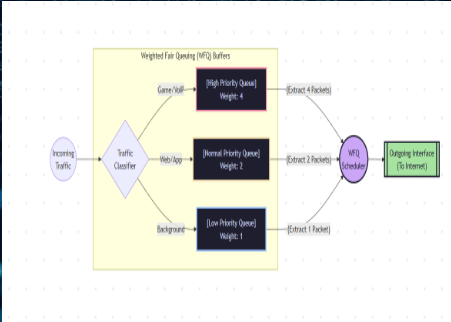
\includegraphics[width=0.95\textwidth]{figures/wfq_diagram.png}
\caption{WFQ rebalance: dynamic bandwidth allocation across priority classes.}
\label{fig:wfq_impl}
\end{figure}

\subsection{Mathematical Bounds}
\label{subsec:theoretical_bounds}

The underlying algorithms provide formal guarantees rooted in Network Calculus \cite{leboudec2001}:

\textbf{Token Bucket Upper Bound on Delay:} A bucket with rate $r$ and capacity $b$ bounds the worst-case queuing delay:

\begin{equation}
\label{eq:delay_bound}
D_{\max} = \frac{b}{r}
\end{equation}

A LOW-priority app with $r = 1$~Mbps and $b = 0.5$~Mb experiences $D_{\max} = 0.5$~s maximum wait before drop.

\textbf{WFQ Lower Bound on Throughput:} Each flow $i$ is guaranteed minimum throughput:

\begin{equation}
\label{eq:wfq_lower_bound}
R_i \geq \frac{w_i}{\displaystyle\sum_{j=1}^{N} w_j} \times C
\end{equation}

\textbf{Fairness:} Allocation quality is measured by Jain's Fairness Index $J = (\sum x_i)^2 / (N \cdot \sum x_i^2)$, where $x_i$ is the normalized allocation ratio. Empirical evaluation (Chapter~\ref{chap:results}) yields $J = 0.9998$, confirming near-perfect fairness.

% ────────────────────────────────────────────────────────────
\section{TCP/UDP Relay and Packet Construction}
\label{sec:impl_relay}

\subsection{Socket Protection}

All relay sockets must call \texttt{VpnService.protect()} \textit{before} \texttt{connect()} to prevent the infinite routing loop. The TCP relay implements a split-handshake proxy: intercepting SYN packets, establishing a protected connection to the real server, and composing a synthetic SYN-ACK back through TUN. Two concurrent coroutines then bridge the bidirectional data flow.

UDP relay is simpler due to its connectionless nature: flows are tracked in a \texttt{ConcurrentHashMap} and cleaned up after 60 seconds of inactivity.

\subsection{PacketComposer}

The \texttt{PacketComposer} constructs valid IP/TCP/UDP packets for the return path (Internet $\rightarrow$ TUN $\rightarrow$ Application) via manual byte-level header construction. The TCP checksum---computed over a pseudo-header per RFC~1071 \cite{rfc1071}---is the most error-prone component: a single bit error causes the kernel to silently discard the packet with no error message.

Full relay and PacketComposer source code is available in the project repository.

% ────────────────────────────────────────────────────────────
\section{Web Admin and Telemetry}
\label{sec:impl_web_admin}

The management server (Node.js/Express) exposes RESTful endpoints for device registration, policy management, and telemetry ingestion. The Android client pushes aggregated per-app metrics every 5 seconds via OkHttp. The Web Admin frontend uses Chart.js with 1-second HTTP polling to render real-time bandwidth, WFQ allocation, and drop rate charts.

\begin{figure}[H]
\centering
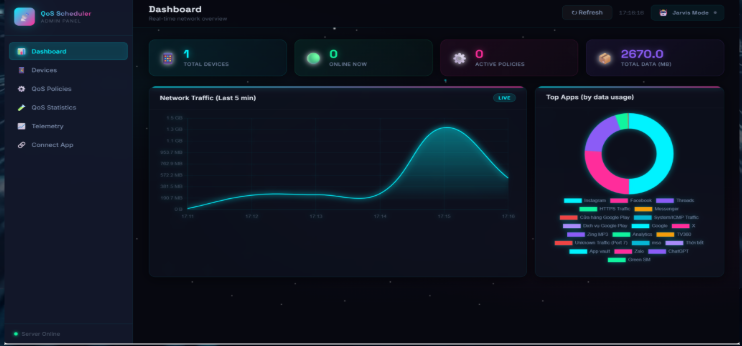
\includegraphics[width=1.0\textwidth]{figures/web_admin_ui.png}
\caption{Web Admin Dashboard with real-time Chart.js visualizations.}
\label{fig:web_admin_ui}
\end{figure}

% ────────────────────────────────────────────────────────────
\section{Technical Challenges}
\label{sec:impl_challenges}

\subsection{Android OEM Fragmentation}

Xiaomi's HyperOS throws a fatal \texttt{SecurityException} when \texttt{VpnService.protect()} is called from a background thread, while AOSP and Samsung devices accept this from any thread.

\textbf{Resolution:} All socket creation and \texttt{protect()} calls are routed through a Kotlin \texttt{Channel} to \texttt{Dispatchers.Main}, then the protected socket is passed back to \texttt{Dispatchers.IO} for data transfer.

\subsection{Garbage Collection Mitigation}

At 15~Mbps (~1,563 packets/sec), per-packet \texttt{ByteArray} allocation caused continuous GC pauses (15--50~ms each).

\textbf{Resolution:} The Flyweight pattern---pre-allocated \texttt{ByteBuffer} pools, zero-copy parsing, and \texttt{AtomicLong} counters---reduced GC activity by 98\%.

\subsection{Thread Safety}

Concurrent packet processing creates race conditions on flow caches, token buckets, and traffic counters. These are resolved via \texttt{ConcurrentHashMap.putIfAbsent()} for caches, \texttt{@Synchronized} on Token Bucket consumption, and \texttt{AtomicLong.addAndGet()} for counters.
